\section{Question 1}

\subsection{Task}
Generate 10 random numbers $y_i$ between -1 and +1. Use these as points $\left(x_i,y_i\right)$ where $x_i=i$ and show them as a scatter plot. Fit a higher order polynomial over these points to generate a pattern of how a random noise would look like. Sample the polynomial to generate about 100 points in the interval $x_1$ to $x_{10}$. Superpose a plot of this data along with original points $\left(x_i,y_i\right)$.  Identify the peaks (location and height) programmatically. Print them out and confirm those with the plot.

\subsection{Solution}

Link to the GitHub repository for this question: \href{https://github.com/Xerefic/MM2090-Solutions/tree/master/Final_Assignment/question_1}{GitHub} \footnote{Repo: \url{https://github.com/Xerefic/MM2090-Solutions/tree/master/Final_Assignment/question_1}}

\subsubsection{Approach}
I used the scikit-learn\footnote{\url{https://scikit-learn.org/stable/}} library to generate a polynomial of degree $n$ and used linear regression to fit the polynomial to the given data. Although this polynomial over fits the given data, it is fine as it retains the randomness of generated coordinates. \\
To find the extrema, I am traversing through the sampled polynomial and identifying the locations where the polynomial attains local maxima or minima. 

\subsubsection{Requirements}
Language of choice: python
\begin{lstlisting}[language=bash]
	pip3 install numpy
	pip3 install matplotlib
	pip3 install sklearn
	pip3 install scipy
\end{lstlisting}

\subsubsection{Output}


\paragraph{Locations of Extremas}

\begin{description}
	\item Maxima at x = 1.4084308430843084 and y = 2.195104229252479
	\item Minima at x = 3.164766476647665 and y = -0.7656559740882756
	\item Maxima at x = 5.218071807180718 and y = -0.19116876616108414
	\item Minima at x = 7.025372537253725 and y = -0.5251533421000687
	\item Maxima at x = 8.292639263926393 and y = -0.2132152812141186
	\item Minima at x = 9.61087108710871 and y = -1.7288452082816121
\end{description}


\subsubsection{Images}

\begin{figure}[!ht]
	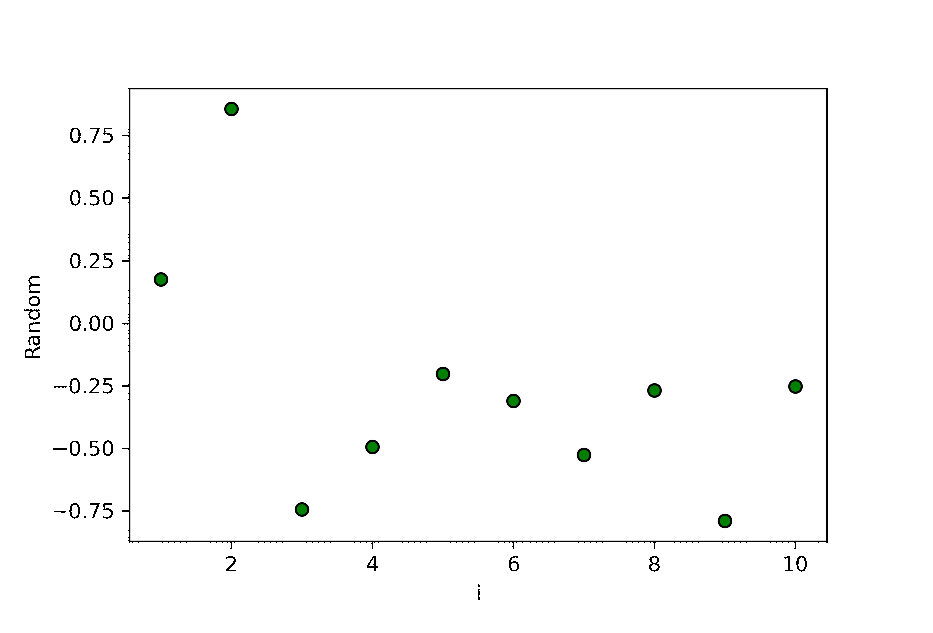
\includegraphics{question_1/Points.eps} 
	\caption{Generated Points}
\end{figure} 

\begin{figure}[!ht]
	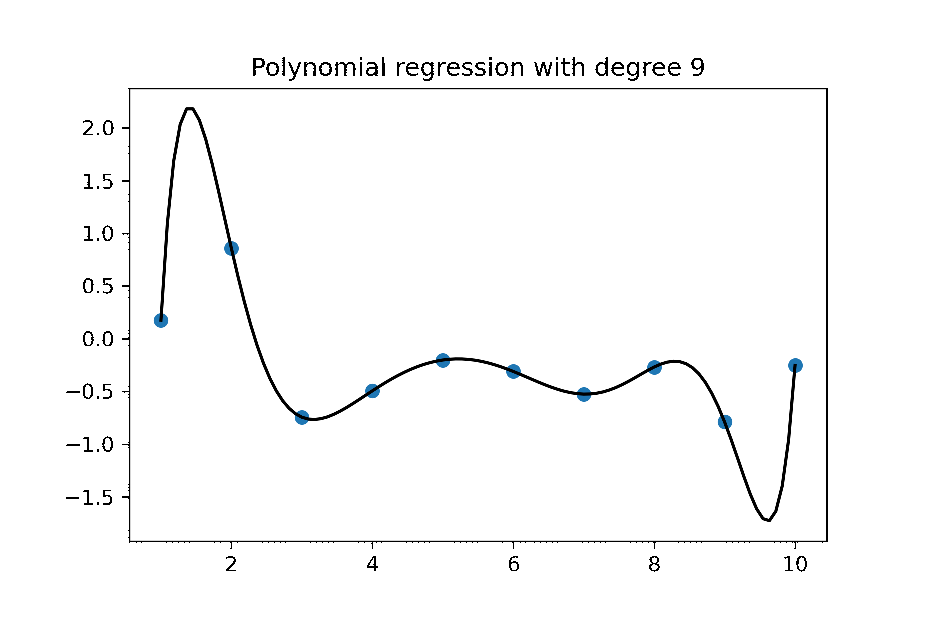
\includegraphics{question_1/Fitted.eps} 
	\caption{Fitted with Polynomial}
\end{figure} 

\clearpage
\subsection{Code}
\lstinputlisting{question_1/question1.py}